% The topic, motivation, the importance of adaptivity 
Consider a dataset $X$ consisting of $n$ independent samples from some unknown population $\dist$.  How can we ensure that the conclusions drawn from $X$ \emph{generalize} to the population $\dist$?  Despite decades of research in statistics and machine learning on methods for ensuring generalization, there is an increased recognition that many scientific findings generalize poorly (e.g. 
\cite{Ioannidis05,GelmanL13}). While there are many reasons a conclusion might fail to generalize, one that is receiving increasing attention is \emph{adaptivity}, which occurs when the choice of method for analyzing the dataset depends on previous interactions with the same dataset~\cite{GelmanL13}.
%
 Adaptivity can arise from many common practices, such as exploratory data analysis, using the same data set for feature selection and regression, and the re-use of datasets across research projects.  Unfortunately, adaptivity invalidates traditional methods for ensuring generalization and statistical validity, which assume that the method is selected independently of the data. The misinterpretation of adaptively selected results has even been blamed for a ``statistical crisis'' in empirical science~\cite{GelmanL13}.
%  ~\cite{GelmanL13}.

\begin{figure}
    \centering
    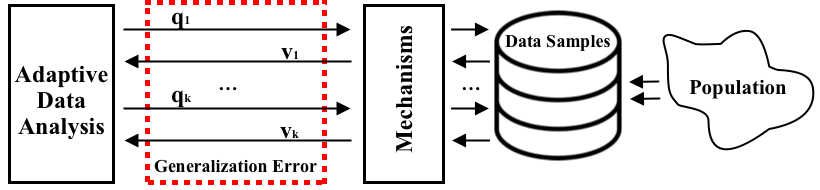
\includegraphics[width=0.7\columnwidth]{overview.png}
    \caption{Overview of our Adaptive Data Analysis model. We have a population that we are interested in studying, and a dataset containing individual samples from this population. The adaptive data analysis we are interested in running has access to the dataset through queries of some pre-determined family (e.g., statistical or linear queries) mediated by a mechanism. This mechanism uses randomization to reduce the generalization error of the queries issued to the data.}
    \label{fig:adaptivity-model-overview}
\vspace{-0.5cm}
\end{figure}

A line of work initiated by \citet{DworkFHPRR15}, \citet{HardtU14} posed the question: Can we design \emph{general-purpose} methods that ensure generalization in the presence of adaptivity, together with guarantees on their accuracy?  The idea that has emerged in these works is to use randomization to help ensure generalization. Specifically, these works have proposed to mediate the access of an adaptive data analysis to the data by means of queries from some pre-determined family (we will consider here a specific family of queries often called "statistical" or "linear" queries) that are sent to a  \emph{mechanism} which uses some randomized process to guarantee that the result of the query does not depend too much on the specific
sampled dataset. This guarantees that the result of the queries generalizes well. This approach is described in Fig.~\ref{fig:adaptivity-model-overview}.  
This line of work has identified many new algorithmic techniques for ensuring generalization in adaptive data analysis, leading to algorithms with greater statistical power than all previous approaches. Common methods proposed by these works include, the addition of noise to the result of a query, data splitting, using sampling methods, etc. Moreover, these works have also identified problematic strategies for adaptive analysis, showing limitations on the statistical power one can hope to achieve. Subsequent works have then further extended the methods and techniques in this approach and further extended the theoretical underpinning of this approach, e.g.~\cite{dwork2015reusable,dwork2015generalization,BassilyNSSSU16,UllmanSNSS18,FeldmanS17,jung2019new,SteinkeZ20,RogersRSSTW20,DaganK22,Blanc23}.


A key development in this line of work is that the best method for ensuring generalization in an adaptive data analysis depends to a large extent on the number of \emph{rounds of adaptivity}, the depth of the chain of queries. As an informal example, the program $x \leftarrow q_1(D);y \leftarrow q_2(D,x);z \leftarrow q_3(D,y)$ has three rounds of adaptivity, since $q_2$  depends on $D$ not only directly because it is one of its input but also via the result of $q_1$, which is also run on $D$, and similarly,  $q_3$ depends on $D$ directly but also via the result of $q_2$, which in turn depends on the result of $q_1$. The works we discussed above showed that, not only does the analysis of the generalization error depend on the number of rounds, but knowing the number of rounds actually allows one to choose methods that lead to the smallest possible generalization error. 
For instance, these works showed that when an adaptive data analysis uses a large number of rounds of adaptivity, then a low generalization error can be achieved by the Gaussian mechanism  
adding to the result of each query Gaussian noise scaled to the number of rounds. When instead  an adaptive data analysis uses a small number of rounds of adaptivity then a low generalization error can be achieved by using more specialized methods, such as the data splitting mechanism or the reusable holdout technique from~\citet{DworkFHPRR15}.
% \detailed{To better understand this idea, we show in Fig.~\ref{fig:generalization_errors} two experiments showcasing these situations. More precisely, in Fig.~\ref{fig:generalization_errors}(a) we show the results of a specific analysis\footnote{We will use formally a program implementing this analysis (Fig.~\ref{fig:overview-example}) as a running example in the rest of the paper.} with two rounds of adaptivity. This analysis can be seen as a classifier which first runs 500 non-adaptive queries on the first 500 attributes of the data, looking for correlations between the attributes and a label, and then runs one last query which depends on all these correlations. Without any mechanism the generalization error is pretty large, and the lower generalization error is achieved when the data-splitting method is used. 
% In Fig.~\ref{fig:generalization_errors}(b), we show the results of a specific analysis\footnote{We will present this analysis formally in Section~\ref{sec:examples}.} with four hundreds rounds of adaptivity. This analysis can be seen as a classifier which at each step runs an adaptive query based on the result of the previous ones. Again, without any mechanism the generalization error is pretty large, and the lower generalization error is achieved when the Gaussian noise is used.}
% \highlight{TO DO: A more detailed explanation of the three adpativity mechanisms}.
% To better understand this idea, we show in Fig.~\ref{fig:generalization_errors} three experiments showcasing these situations. More precisely, in Fig.~\ref{fig:generalization_errors}(a) we show the results of a specific analysis\footnote{We will use formally a program implementing this analysis (Fig.~\ref{fig:overview-example}) as a running example in the rest of the paper.} with two rounds of adaptivity. This analysis can be seen as a classifier which first runs 400 non-adaptive queries on the first 400 attributes of the data, looking for correlations between the attributes and a label, and then runs one last query which depends on all these correlations. Without any mechanism the generalization error of the last query is pretty large, and the lower generalization error is achieved when the data-splitting method is used. Fig.~\ref{fig:generalization_errors}(c) shows how this situation also changes with the number of queries. Specifically, it shows the root mean square error of the last \emph{adaptive} query when the number of queries varies. This also highlights the fact that different mechanisms, for the same analysis, produce results with different generalization errors.
% In Fig.~\ref{fig:generalization_errors}(a) and Fig.~\ref{fig:generalization_errors}(c) we  use the same analysis but different data sizes. This is mostly to account for 
% the fact that we run many more queries in Fig.~\ref{fig:generalization_errors}(c). Using a larger data set in Fig.~\ref{fig:generalization_errors}(c) also changes the magnitude of the error. 

To better understand this idea, we show in Fig.~\ref{fig:generalization_errors} three experiments showcasing these situations: 
% \highlight{Fig.~\ref{fig:generalization_errors}(a) shows the generalization errors of one adaptive data analysis program with the adaptivity $2$ when no mechinism(marked as overfitted), Gaussian mechanism(guassian noise) and Data splitting mechanism(data splitting) are applied;
%  Fig.~\ref{fig:generalization_errors}(b) shows the generalization errors of one adaptive data analysis under similar three conditions as Fig.~\ref{fig:generalization_errors}(a), the difference is the adapativity is $400$ instead of $2$;
%   Fig.~\ref{fig:generalization_errors}(c) shows how the generalization errors also change along with the number of queries when various mechanisms are applied.} 
% More precisely,  
In Fig.~\ref{fig:generalization_errors}(a) we show the results of a specific analysis\footnote{We will use formally a program implementing this analysis (Fig.~\ref{fig:overview-example}) as a running example in the rest of the paper.} 
with two rounds of adaptivity.
\review{Making Figure 2 more legible, and including a more detailed explanation of the different adaptivity mechanisms.}
 \highlight{This analysis can be seen as a classifier for a population where individuals samples consist of 400 attributes and 1 label. Using a dataset representing a sample from this population, this analysis first runs 400 non-adaptive queries on the first 400 attributes of the dataset,
  computing correlations between each attribute and the label. Then, it runs the last query depending on all these correlations. The adaptivity of this analysis is $2$ because only the last query relies on the results of the previous queries' results. 
  Without any mechanism the generalization error of the last query may be pretty large, and we can achieve lower generalization error by using the data-splitting method. 
  In Fig.~\ref{fig:generalization_errors}(c), we use the same data analysis program as in Fig.~\ref{fig:generalization_errors}(a). It runs over a dataset with larger data size and shows only the root mean square error of the last \emph{adaptive} query when the 
total query number varies along the x-axis. This figure is meant to show how the total number of queries also affect the generalization error.
Fig.~\ref{fig:generalization_errors}(c) also highlights the fact that different mechanisms, for the same analysis, produce results with different generalization errors, and
using a larger data set changes the magnitude of the error. } 
In Fig.~\ref{fig:generalization_errors}(b), we show the results of a specific analysis\footnote{We will present this analysis formally in Section~\ref{sec:examples}.} with four hundred rounds of adaptivity.
At each step, this analysis runs an adaptive query based on the results of the previous ones. Without any mechanism, the generalization error of most of the queries is pretty large, and this error can be lowered by using Gaussian noise. 
\highlight{Overall, in Fig.~\ref{fig:generalization_errors} we use  three different mechanisms: the Gaussian mechanism which adds tp the result of each query Gaussian noise; the Data Splitting mechanism
that splits the data into a few parts on which runs independently the different queries; the Thresholdout mechanism that uses the reusable holdout technique from~\citet{DworkFHPRR15}.  }
{\small
\begin{figure}
\centering
\begin{subfigure}{.322\textwidth}
\begin{centering}
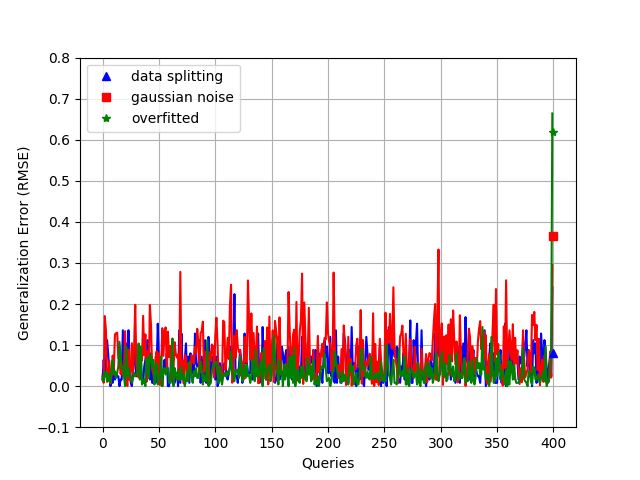
\includegraphics[width=1.0\textwidth]{tworound.png}
\caption{}
\end{centering}
\end{subfigure}
\quad
\begin{subfigure}{.322\textwidth}
\begin{centering}
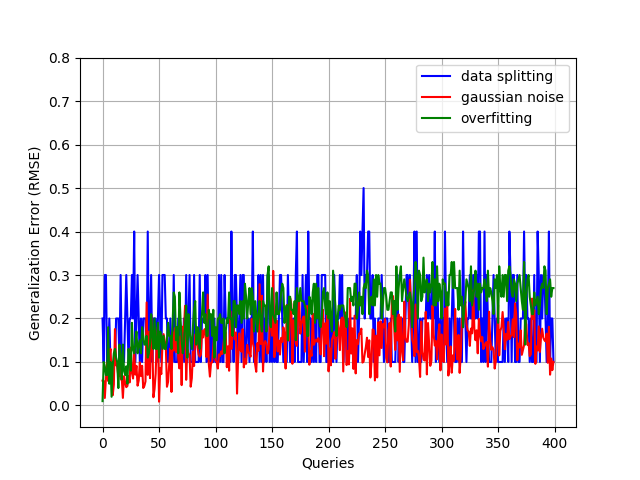
\includegraphics[width=1.0\textwidth]{multipleround.png}
\caption{}
\end{centering}
\end{subfigure}
\begin{subfigure}{.322\textwidth}
\begin{centering}
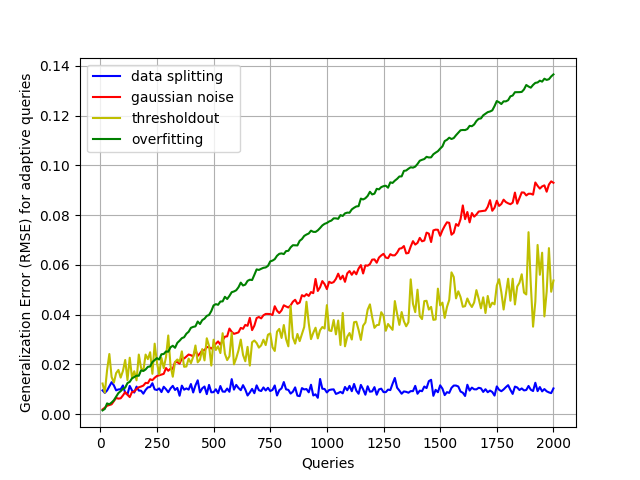
\includegraphics[width=1.0\textwidth]{twoRounds-rmse-fourmechs.png}
\caption{}
\end{centering}
\end{subfigure}
\vspace{-0.2cm}
 \caption{
 The generalization errors of two adaptive data analysis examples, under different choices of mechanisms.
 (a)  2 rounds adaptivity. 
 (b)  400 rounds adaptivity.
 (c) 2 rounds adaptivity with varied query numbers.
}
\label{fig:generalization_errors}
\vspace{-0.2cm}
\end{figure}
}
%gap

This scenario motivates us to explore the design of program analysis techniques that can be used to estimate the number of \emph{rounds of adaptivity} that a program implementing a data analysis can perform. These techniques could be used to help a data analyst in the choice of the mechanism to use,
and they
could ultimately be integrated into a tool for adaptive data analysis such as the \emph{Guess and Check} framework by~\citet{RogersRSSTW20}. 

The first problem we face is \emph{how to formally define} a model for adaptive data analysis which is general enough to support the methods we discussed above and which would permit to formulate the notion of adaptivity these methods use. We take the approach of designing a programming framework for submitting queries to some \emph{mechanism} giving access to the data mediated by one of the techniques we mentioned before, e.g., adding Gaussian noise, randomly selecting a subset of the data, using the reusable holdout technique, etc. In this approach, a program models an \emph{analyst} asking a sequence of queries to the mechanism. The mechanism runs the queries on the data applying one of the methods above and returns the result to the program. The program can then use this result to decide which query to run next. Overall, we are interested in controlling the generalization error of the query results returned by the mechanism, by means of the adaptivity. 

The second problem we face is \emph{how to define the adaptivity of a given program}.
Intuitively, a query $Q$ may depend on another query $P$, if there are two values that $P$ can return which affect in different ways the execution of $Q$. 
For example, as shown in \cite{dwork2015reusable}, and as we did in our example in Fig.~\ref{fig:generalization_errors}(a), one can design a machine learning algorithm for constructing a classifier which first computes each feature's correlation with the label via a sequence of queries, and then constructs the classifier based on the correlation values. If one feature's correlation changes, the classifier depending on features is also affected.  
This notion of dependency builds on the execution trace as a \emph{causal history}. In particular, we are interested in the history or provenance of a query up until this is executed, and we are not then concerned about how the result is used --- except for tracking whether the result of the query may further cause some other queries. This is because we focus on the generalization error of queries and not their post-processing. % 
To formalize this intuition as a quantitative program property,
we use a trace semantics recording the execution history of programs on some given input --- and we create a dependency graph, where the dependency between different variables (queries are also assigned to variables) is explicit and tracks which variable is associated with a query request. We then enrich this graph with weights describing the number of times each variable is evaluated in a program evaluation starting with an initial state. The adaptivity is then defined as the length of the walk visiting the most query-related variables on this graph\footnote{Formally, graphs will be well-defined only for terminating programs, this will guarantee that the walk is finite}. In other words, we define adaptivity as a \emph{quantitative form of program dependency}.

% \jl{ 
% To define adaptivity in our programming framework, we consider a weighted dependency graph over variables assigned in the program, where each edge is built by a semantics dependency relation between these variables. The dependency relation relies on the trace semantics of our programming framework which records the execution history of programs implementing adaptive data analysis. 
% %The novelty comes from the definition of relation of dependency between nodes, which consists of the edge in the graph. For now, we can think of each node is associated with a variable, storing the value assigned to its variable 
% }
% \jl{The general idea beneath this dependency relation is that modifying the value of some variable in an execution trace will later affect the following execution trace.
% By tracking if a variable is assigned by a query or not, we are able to distinguish whether one query may depend on the other.}

The third problem we face is \emph{how to estimate the adaptivity of a given program}. 
The adaptive data analysis model we consider and our definition of adaptivity suggest that for this task we can use a  program analysis that is based on some form of dependency analysis. This analysis needs to take into consideration:
1) the fact that, in general, a query $Q$ is not a monolithic block but rather it may depend, through the use of variables and values, on other parts of the program. Hence, it needs to consider some form of data flow analysis. 
2) the fact that, in general, the decision on whether to run a query or not may depend on some other value. Hence, 
 it needs to consider some form of control flow analysis.
 3) the fact that, in general, we are not only interested in whether there is a dependency or not, but in the length of the chain of dependencies. Hence, it needs to consider some quantitative information about the program dependencies. 
 
To address these considerations and be able to estimate a sound upper bound on the adaptivity of a program, 
we develop a static program analysis algorithm, named {\THESYSTEM}, which combines data flow and control flow analysis with reachability bound analysis~\cite{GulwaniZ10}. This combination gives tighter bounds on the adaptivity of a program than the ones one would achieve by directly using the data and control flow analyses or the ones that one would achieve by directly using reachability bound analysis techniques alone. We evaluate {\THESYSTEM} on a number of examples showing that it is able to efficiently estimate precise upper bounds on the adaptivity of different programs. 
All the proofs and extended definitions can be found in the supplementary material.

To summarize, our work aims at the design of a static analysis for programs implementing adaptive analysis that can estimate their rounds of adaptivity. Specifically, our contributions are:
\begin{enumerate}
    \item A programming framework for adaptive data analyses where programs represent analysts that can query generalization-preserving mechanisms mediating the access to some data. 
    \item 
    A formal definition of the notion of adaptivity under the analyst-mechanism model,
    built on a variable-based dependency graph constructed using sets of program execution traces.
    \item 
    A static program analysis algorithm {\THESYSTEM} combining data flow, control flow and  reachability bound analysis in order to provide tight bounds on the adaptivity of a program.
    \item A soundness proof of the program analysis showing that the adaptivity estimated by {\THESYSTEM} bounds the true adaptivity of the program. 
    \item A prototype implementation of {\THESYSTEM} and an experimental evaluation showing its accuracy and efficiency of the adaptivity estimation on several examples.  
    We also provide an evaluation showing how the generalization error of several real-world data analyses can be effectively reduced by using the information provided by {\THESYSTEM}.
\end{enumerate}
